\documentclass[tikz,convert,crop,boder=100px]{standalone}
% vim:noet:sts=2:ts=2:sw=2:smarttab:tw=120
\usepackage{pgfplots}
\usetikzlibrary{arrows,shapes,positioning,calc}

\begin{document}
	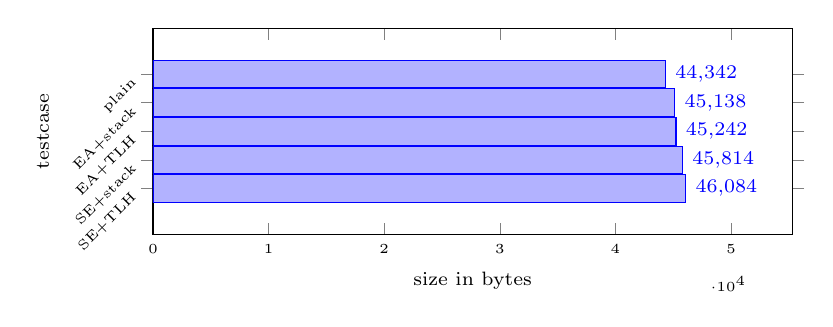
\begin{tikzpicture}[font=\scriptsize]
		\begin{axis}[
			width=.8\textwidth,
			height=4.2cm,
			xbar,
			xlabel=size in bytes,
			ylabel=testcase,
			enlarge y limits=0.4,
			xmin=0,
			enlarge x limits={0.2,upper},
			symbolic y coords={SE+TLH, SE+stack, EA+TLH, EA+stack, plain},
			ytick=data,
			y tick label style={rotate=45, anchor=east},
			nodes near coords,
			nodes near coords align={horizontal},
			legend style={draw={none}, fill={none}, at={(0.5, 0.99)}, anchor={north}, legend columns=-1},
			legend cell align=left,
			label style={font=\scriptsize},
			tick label style={font=\tiny},
			legend style={font=\tiny}
		]
		  % all allocations
			\addplot coordinates {%
				(46084,SE+TLH)
				(45814,SE+stack)
				(45242,EA+TLH)
				(45138,EA+stack)
				(44342,plain)
			};
			%\addlegendentry{\;on-the-go\;}
		\end{axis}
	\end{tikzpicture}
\end{document}
